\documentclass{article}

\PassOptionsToPackage{numbers, square}{natbib}
\usepackage[final]{nips_2017}

\usepackage[utf8]{inputenc}
\usepackage[T1]{fontenc}
\usepackage{amsmath}
\usepackage{amssymb}
\usepackage{hyperref}
\usepackage{graphicx}
\usepackage{subcaption}
\usepackage{booktabs}
\usepackage{float}
\raggedbottom
\usepackage[labelfont=bf]{caption}
\setcitestyle{square, comma, numbers}

\title{Compressing Chain-of-Thought Length in Small Language Models via GRPO}

\author{
  \textbf{Filip Łazowski} \\
   University of Warsaw \\
  \texttt{fl448341@students.mimuw.edu.pl}
  \And
  \textbf{Bartłomiej Cupiał}\thanks{Supervisor of the project} \\
   University of Warsaw \\
  \texttt{b.cupial@uw.edu.pl}
}

\begin{document}

\maketitle
\setcounter{footnote}{0}
\begin{abstract}
This work presents a reinforcement learning approach to compress Chain-of-Thought reasoning in small language models without degrading accuracy. Shortening reasoning through prompt engineering lowers mathematical performance, whereas enforcing brevity via a naive length penalty in Group Relative Policy Optimization triggers reward hacking and policy collapse. To resolve this, the training objective is regularized against the base model to ensure controlled compression. Evaluated on the GSM8K dataset with the Qwen2.5-0.5B model, the optimized policy achieves 49 percent accuracy at a mean length of 222 tokens. This improves accuracy by 9 percentage points while reducing reasoning length by 23 percent compared to the untrained baseline. Code is available at \href{https://github.com/fl448341/grpo_cot_compression}{\textit{GitHub}}.
\end{abstract}

\section{Introduction}
Language models use Chain-of-Thought reasoning to decompose complex problems into simpler, smaller tasks \cite{wei2022chain, zhou2022least}. A common intuition in the field has been that longer and more detailed reasoning steps lead to better performance, particularly for mathematically difficult tasks \cite{fu2023complexity, jin2024impact}. However, recent research demonstrates that reasoning performance does not consistently improve as chains grow longer, and instead, task accuracy typically follows an inverted U-shaped curve with respect to CoT length \cite{wu2025when}. While accuracy initially improves as the task is appropriately decomposed, it eventually degrades in longer chains due to error accumulation \cite{wu2025when}.

To optimize CoT length in small models, the Group Relative Policy Optimization \cite{shao2024deepseekmath} was employed. Unlike capable models that naturally reduce reasoning length during standard reinforcement learning \cite{wu2025when}, enforcing brevity on small models via a length penalizing reward in GRPO introduces optimization barriers. Specifically, it triggers reward hacking mechanism \cite{skalse2022defining}, where the policy collapses by bypassing reasoning entirely to maximize the brevity reward. To address this issue and investigate the trade-off between CoT length and accuracy, this work proposes a two-phase framework: first establishing a reasoning baseline through prompt engineering, and second stabilization of length penalized GRPO.

\subsection{Experimental Setup}
The model selected for all experiments is Qwen2.5-0.5B-Instruct \cite{qwen2.5_technical_report}, evaluated on the GSM8K dataset \cite{cobbe2021}. For the reinforcement learning stage, the training pipeline utilizes a modified TinyZero \cite{tinyzero} framework, adapted to support custom reward logic and length penalization. All computations are executed on a RunPod instance with a single NVIDIA RTX 4090 GPU (24GB VRAM).

\section{Phase 1: Empirical Analysis of CoT Length and Prompting Baseline}
The first phase explores the relation between CoT length and accuracy for the base model, and introduces an untrained baseline for shortening reasoning through prompt engineering. All evaluations are performed on the first 200 problems of the GSM8K test split using greedy decoding. Because this model seems to disobey standard response formatting, correctness is scored with a custom extractor that parses different kinds of numeric responses - this avoids the potential false negatives.

\paragraph{Natural baseline and the length-accuracy relationship.}
With empty system prompt, the model scores $41\%$ accuracy with a mean CoT length of $290$ tokens. Partitioning these answers into length quartiles shows a relationship between reasoning length and correctness (Figure~\ref{fig:p1_length}): the shortest quartile (143 - 215 tokens) has $57\%$ of accuracy, whereas the longest quartile (347 - 512 tokens) collapses to $14\%$. This is consistent with the inverted-U behaviour\footnote{Note that pure inverted-U would show if the model wasn't tuned for reasoning, as of now it is not capable of producing straightforward, short answers} reported by \cite{wu2025when}. For this model, length acts as a sign of difficulty, meaning that harder problems cause longer, error prone chains, rather than as a cause of improved performance.

\paragraph{Prompt engineering for brevity.}
Next experiment tested whether reasoning can be shortened by instruction alone. Three brevity oriented system prompts (\textit{brief}, \textit{concise}, \textit{minimal} - Figure \ref{fig:prompts3}) are compared against the baseline (Figure~\ref{fig:p1_prompts}). Prompting does compress the chains, but at a accuracy cost. The \textit{brief} prompt gives the best trade-off, reaching $37\%$ accuracy at $220$ tokens (a~ $\!24\%$ length reduction for a $4$ points accuracy drop), while the \textit{concise} and \textit{minimal} prompts compress to $233$ and $224$ tokens but drop the accuracy to $35\%$ and $36.5\%$ respectively.

\begin{figure}[H]
  \centering
  \begin{minipage}{0.92\linewidth}\small
\begin{verbatim}
"brief":   "Solve the math problem. Think step by step, 
            but keep your reasoning brief."
"concise": "Solve the math problem using as few reasoning steps as possible.
            Be concise, then give the final answer."
"minimal": "Solve the math problem. Give only the minimal reasoning needed,
            then state the final answer."
\end{verbatim}
  \end{minipage}
  \caption{Three system prompts used for the reasoning shortening.}
  \label{fig:prompts3}
\end{figure}

Together, these results define the baseline that the reinforcement learning phase seeks to surpass. Prompt engineering shows that shorter reasoning is attainable only by sacrificing accuracy. Phase 2 investigates whether a length penalized GRPO objective can move beyond this, producing shorter chains at same or higher accuracy.

\begin{figure}[H]
  \centering
  \begin{subfigure}[t]{0.49\linewidth}
    \centering
    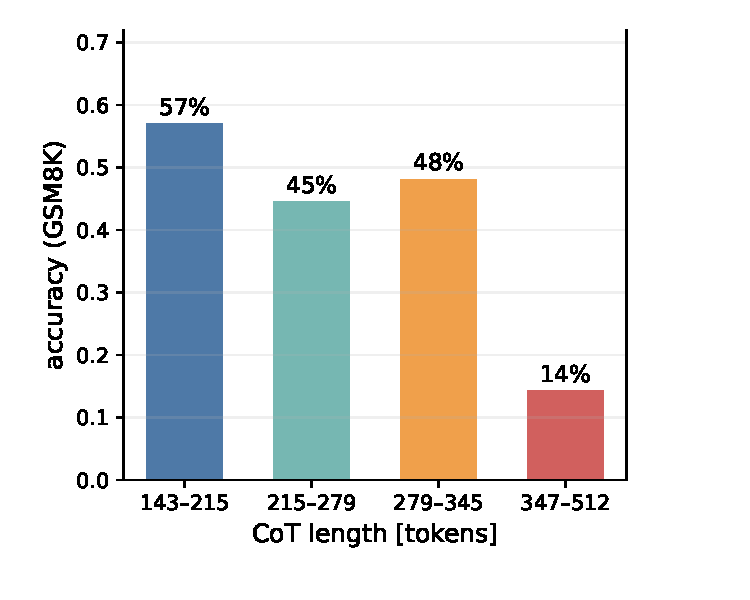
\includegraphics[height=5cm]{figures/fig_phase1_length_acc.pdf}
    \caption{Accuracy by CoT length quartile. The longest answers are the least accurate.}
    \label{fig:p1_length}
  \end{subfigure}\hfill
  \begin{subfigure}[t]{0.49\linewidth}
    \centering
    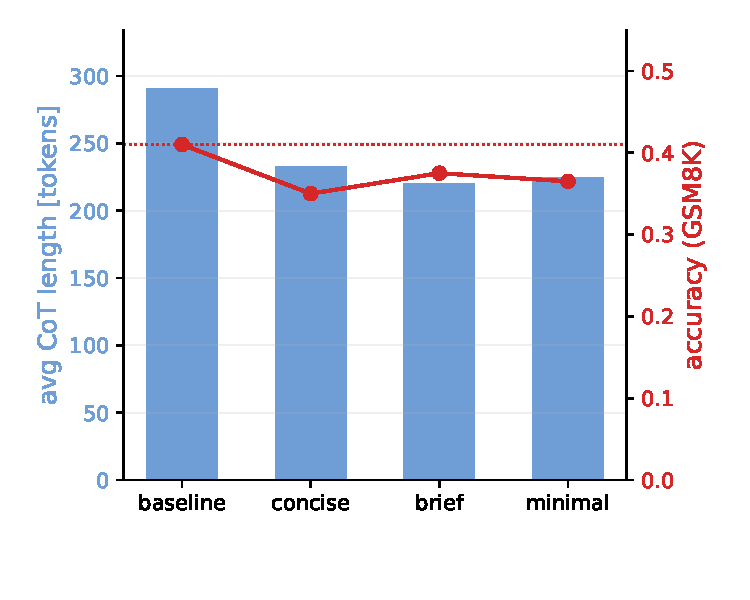
\includegraphics[height=5cm]{figures/fig_phase1_prompts.pdf}
    \caption{Brevity prompts shorten the CoT  but lower accuracy. \textit{Brief} is the best trade-off in the Phase 1.}
    \label{fig:p1_prompts}
  \end{subfigure}
  \caption{Phase 1 on Qwen2.5-0.5B-Instruct / GSM8K.}
  \label{fig:phase1}
\end{figure}

\section{Phase 2: Compressing Reasoning with Length Regularized GRPO}
In Phase 2 a training to shorten the model's reasoning with GRPO occurs. In one training step a batch of $64$ prompts is being sampled and, for each prompt, $G=8$ completions ($o_i$) is generated with temperature sampling ($T=0.7$) from the policy $\pi_{\text{old}}$ that generates this step's completions. Temperature sampling is used so the completions in one group differ rather than give the same answer. Each completion $o_i$ of length $\ell_i$ tokens is scored by a reward that combines correctness with a length penalty,
\[ R_i = \mathbf{1}[\text{correct}_i] \;-\; \lambda\,\frac{\ell_i}{512}, \]
where $\mathbf{1}[\text{correct}_i]$ is $1$ when the answer in $o_i$ is correct and $0$ otherwise. The length is normalized by a constant so that $\lambda$ means the same thing across runs. Because GRPO does not use a critic, the group itself acts as one - within each group of $8$ the reward produce the advantage $\hat{A}_i=(R_i-\mathrm{mean}_g)/(\mathrm{std}_g+\varepsilon)$ and assign it to every token of $o_i$. The group of size $8$ was chosen to  provide stable signal and reducing computing cost (on single GPU),  and also to produce diverse completions - if all completions are all wrong (or all correct) $\lambda$ terms cancels out in the group's advantage and its value doesn't matter in this group. Then a single gradient update on the batch is done (one minibatch, one epoch) that maximizes the GRPO objective of DeepSeek \cite{shao2024deepseekmath},


\begin{equation*}
\begin{aligned}
\mathcal{J}_{\mathrm{GRPO}}(\theta) &= \mathbb{E}_{q \sim P(Q),\,\{o_i\}\sim\pi_{\theta_{\mathrm{old}}}}\!\left[\frac{1}{G}\sum_{i=1}^{G}\frac{1}{|o_i|}\sum_{t=1}^{|o_i|} L_{i,t}\right], \\[2pt]
L_{i,t} &= \min\!\big(\rho_{i,t}\,\hat A_{i,t},\ \mathrm{clip}(\rho_{i,t},\,1{-}\epsilon,\,1{+}\epsilon)\,\hat A_{i,t}\big)\;-\;\beta\,\mathbb{D}_{\mathrm{KL}}\!\left[\pi_\theta\,\|\,\pi_{\mathrm{ref}}\right].
\end{aligned}
\end{equation*}
Here $\rho_{i,t}=\pi_\theta(o_{i,t}\mid q,o_{i,<t})/\pi_{\theta_{\mathrm{old}}}(\cdot)$ is the importance ratio, $\hat A_{i,t}=\hat A_i$ is advantage for every token $t$ of $o_i$ (the reward is a single scalar per answer), $\epsilon$ is the clip ratio, and $\beta\ge 0$ the KL coefficient. Since exactly one gradient update is run per rollout, $\rho_{i,t}=1$: the clip is never used and one training step simply is a group relative policy gradient with a KL penalty - $\mathbb{D}_{\mathrm{KL}}$ (Schulman's low-variance k3 estimator \cite{k3}).

\paragraph{A sign issue.}\label{sign}
The KL term above is meant to penalize divergence from the base, with $\beta\ge 0$. It was found that the TinyZero implementation that was used combines this term into the loss with the wrong sign, so that a positive \texttt{kl\_loss\_coef} ends up rewarding divergence rather than penalizing it, which was the default for the GRPO. It was verified in the implementation and directly on the $\lambda=0$ with a positive coefficient ($+5$) which drives the policy away from the $\pi_{\text{ref}}$ and collapses accuracy to $13.9\%$. Whereas with a negative coefficient ($-5$) KL is near zero with accuracy $42.5\%$.

All accuracy and length numbers below use the same greedy-decoded GSM8K test split as Phase 1, but with the training prompt, which append system prompt to reason step by step and give the final answer after a \texttt{\#\#\#\#}. With this prompt the untrained base model scores $40.0\%$ at a mean of $287$ tokens (median $265$), one point below the $41\%$ it scores with the empty prompt in Phase 1.

\paragraph{The reward hacking.}
First runs trained for $50$ steps. With any positive $\lambda$ this leads to the model not learning to reason more briefly, it learns to skip reasoning instead. It finds that generating a random number in the response collects the length reward, and accuracy drops almost to zero - and the more accuracy drops the faster it degrades - see $\lambda$ term cancelation above).

Figure~\ref{fig:p2_collapse} shows this on the $50$-step run: the mean response length drops from about $350$ tokens to about $5$, while the KL from the base model rises from $0$ to about $7$ (specifically it's $\texttt{kl\_loss}$ metrics). This is known as reward hacking, and in our case the length term is optimized at the cost of the accuracy. Note that the KL is measured against the reference, so its spike happens together with the length compression and partly measures how far the policy has moved, not correctness on its own. It still acts as a good metrics for testing whether model has degraded too much and differs from the base model, which one would like to avoid to some extent.

\begin{figure}[H] 
  \centering
  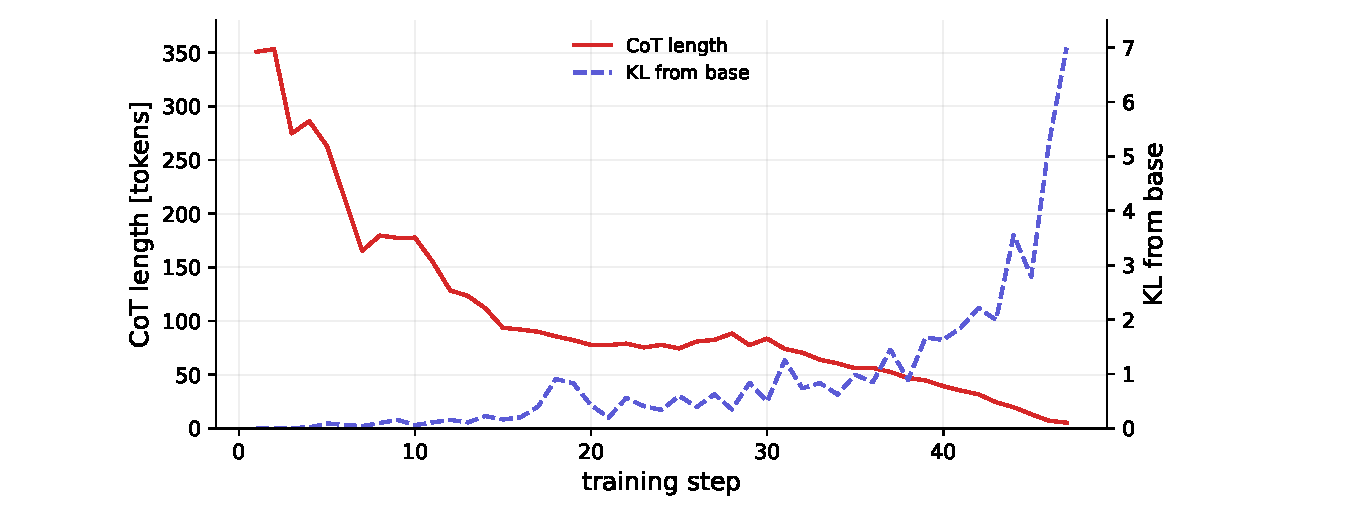
\includegraphics[width=\linewidth]{figures/fig_p2_collapse.pdf}
  \caption{Reward hacking on the 50 steps run ($\lambda=0.1$, default $\beta$): the mean CoT length collapses to a few tokens while the KL from the base explodes to about $7$, meaning that the policy stops reasoning to collect the length reward.}
  \label{fig:p2_collapse}
\end{figure}

\paragraph{Controlled compression.}
The fix for reward hacking has two parts. Firstly, setting correct KL penalty (see \ref{sign}), which keeps the policy close to a base model so it shortens the CoT in a controlled way instead of collapsing - this part will be referred as KL anchor. Second part is to lower the training loop steps, because even with the KL anchor the policy eventually degrades too much. It is set specifically to 15 steps, which has proved to work the best during test runs. Figure~\ref{fig:kneg_dynamics} shows the training dynamics for $\lambda\in\{0, 0.01,0.05,0.1\}$ at $\beta=0.01$. 
The most important conclusion from these graphs is that the CoT length drops steadily for positive lambdas, while the KL does not increase too much compared to former runs without KL anchor. Reward is not that important to use as a metrics, as it depends strongly on the noise caused by sampling - what's more important is that the model doesn't degrade too much so the reward for responses could still have a positive impact on model's policy update. Note that for $\lambda = 0$ length stays at the base and its KL barely change, so the compression and the KL climb in the other runs are driven by the length reward and that no signal collapses, in contrast to a length penalty without the anchor (Figure~\ref{fig:p2_collapse}).

\begin{figure}[H]
  \centering
  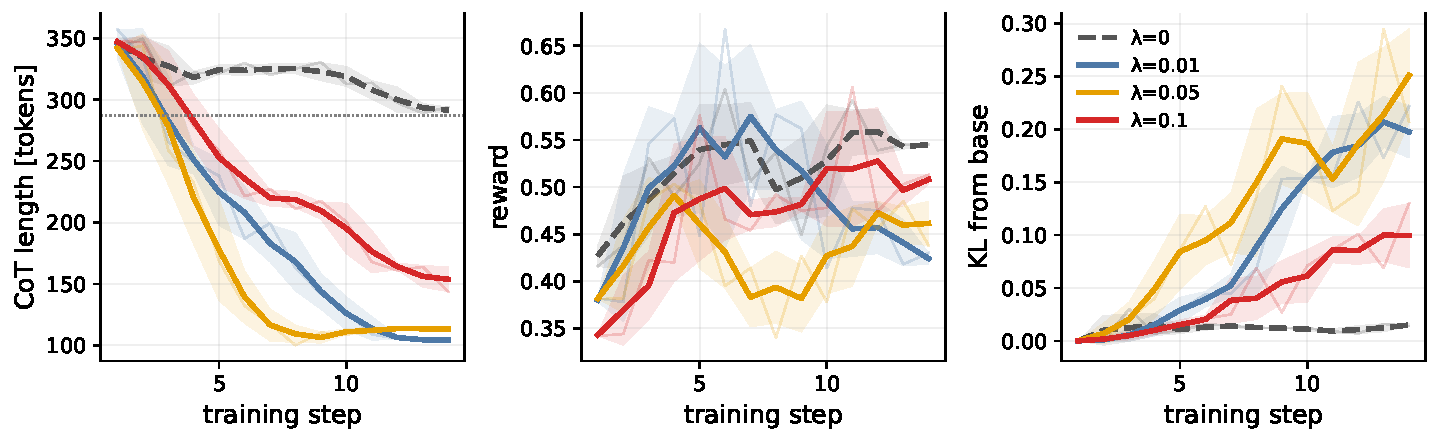
\includegraphics[width=\linewidth]{figures/kneg_dynamics.pdf}
  \caption{Chosen metrics during GRPO training for each $\lambda$ at $\beta=0.01$ ($\texttt{kl\_loss\_coef}=-0.01$). Left: response length (dotted line is the Phase 1 baseline). Middle: reward. Right: KL from base. Signle run noise - solid line is a rolling mean and band is rolling std.}
  \label{fig:kneg_dynamics}
\end{figure}

\subsection{Evaluation and trade-offs}
Because the KL anchor tries to keep the model at the base while the length reward pulls the other way, the two need to be balanced. In Figure~\ref{fig:kneg_steps} every $\lambda$ first increases above the base model, peaking around $45$ to $50\%$ at steps $3$ to $6$, then later accuracy is traded for more CoT compression. Both $\lambda=0.01$ and $\lambda=0.1$ keep accuracy above the base while compressing, $\lambda=0.05$ compresses fastest but overshoots, dropping below the base by step $6$.

\begin{figure}[H]
  \centering
  \begin{subfigure}[t]{0.49\linewidth}
    \centering
    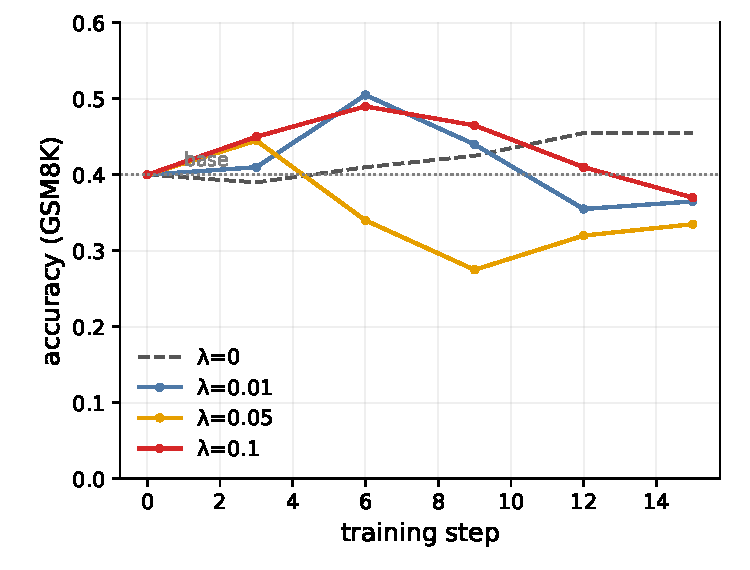
\includegraphics[width=\linewidth]{figures/kneg_accuracy_steps.pdf}
    \caption{Accuracy vs.\ step. The $\lambda>0$ runs rise above the base ($40\%$) at the begining. The $\lambda=0$ keeps around the baseline and never compresses.}
    \label{fig:kneg_acc}
  \end{subfigure}\hfill
  \begin{subfigure}[t]{0.49\linewidth}
    \centering
    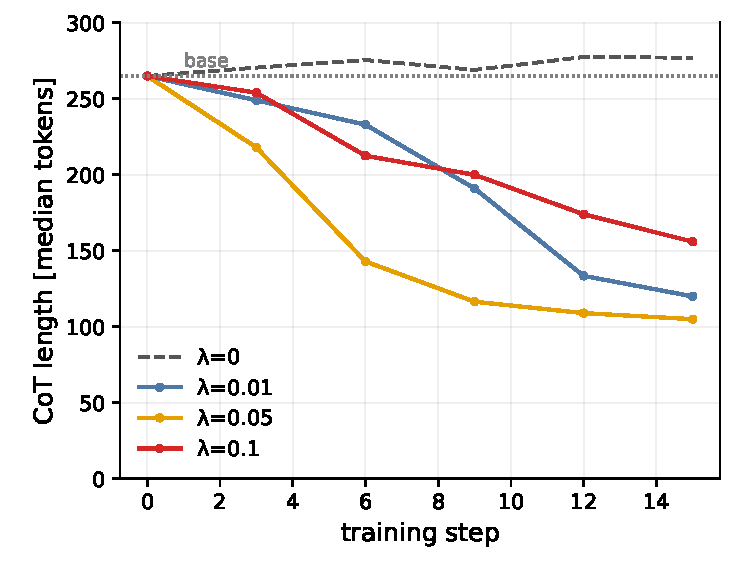
\includegraphics[width=\linewidth]{figures/kneg_length_steps.pdf}
    \caption{Median CoT length vs. step. The $\lambda=0$ stays at the base, while $\lambda>0$ runs compress the CoT.}
    \label{fig:kneg_len}
  \end{subfigure}
  \caption{Evaluation of length penalized GRPO with a KL penalty on GSM8K test split ($\beta=0.01$, $\texttt{kl\_loss\_coef}=-0.01$), $\lambda\in\{0.01,0.05,0.1\}$, $15$ steps. The compression is controlled and trades off against accuracy, the useful checkpoints are early to mid training.}
  \label{fig:kneg_steps}
\end{figure}

\paragraph{What matters.} Note that because the training loop is shortened, the metrics can be noisy and the exact values should not be overinterpreted. Restriction to 15 steps casuses each $\lambda$ to not affect the compression rate accordingly. This is visible on the charts, where $\lambda=0.1$ doesn't compress much faster than smaller ones. At this scale, the choice of the $\lambda$ is not that important, as long as $\lambda > 0$, which successfully guide the policy towards CoT shortening without losing much accuracy. Relation where a larger $\lambda$ causes rapid compression, only shows up during longer trainings, which of course triggers reward hacking and model degradation. Because the goal was to find a practical trade-off, this work focused on finding the best stable configuration for this small model.


\paragraph{Proper comparison.} Table~\ref{tab:kneg} lists the best checkpoints. The highest accuracy for $\lambda=0.1$ at step $6$, reaches $49.0\%$ at a mean of $222$ tokens ($9$ points above the Phase 2 base and $23\%$ shorter). Trading accuracy for length, $\lambda=0.01$ at step $9$ gives $44.0\%$ at $192$ tokens and $\lambda=0.1$ at step $12$ reaches $188$ tokens while holding the Phase 2 base accuracy ($40\%$). The contrast with Phase 1 shows that GRPO works better for compressing CoT without losing accuracy. 

\begin{table}[H]
  \centering
  \caption{Evaluation on GSM8K. Best chosen.}
  \label{tab:kneg}
  \begin{tabular}{llcc}
    \toprule
    \textbf{Phase} & \textbf{Configuration} & \textbf{Accuracy} & \textbf{Mean length} \\
    \midrule
    \textbf{1: Prompting} & Empty & $41.0\%$ & $290$ \\
                          & \textit{Brief} prompt   & $37\%$ & $220$ \\
    \midrule
    \textbf{2: GRPO}      & Untrained base          & $40.0\%$ & $287$ \\
                          & $\lambda=0.1$ (step 6)  & $\mathbf{49.0\%}$ & $222$ \\
                          & $\lambda=0.01$ (step 9) & $44.0\%$ & $192$ \\
                          & $\lambda=0.1$ (step 12) & $41.0\%$ & $\mathbf{188}$ \\
    \bottomrule
  \end{tabular}
\end{table}



\paragraph{Evaluation example.}
Figure~\ref{fig:kneg_example} shows three different policies on one problem. The base model generete the solution with $223$ tokens, with numbered steps and full sentences. The GRPO policy ($\lambda=0.1$, step $9$) reaches the same correct answer in $54$ tokens keeping reasoning, but dropping the redundancy. The third policy without KL anchor generate the wrong number \texttt{11} with no reasoning, which is collapse that the KL anchor stops.

\begin{figure}[H]
  \centering
  \begin{minipage}{0.7\linewidth}\small
\begin{verbatim}
Problem (idx 91):  Jan has three times the number of pets as Marcia.
Marcia has two more pets than Cindy. If Cindy has four pets, how many
total pets do the three have?                    (Correct answer: 28)

[base model, 223 tokens, correct]
  To find out how many pets Jan, Marcia, and Cindy have in total, we
  need to follow these steps:
   1. Determine how many pets Marcia has.
   2. Use that information to determine how many pets Jan has.
   3. Add up all the pets.
  First, ... Marcia has 4 + 2 = 6 pets.
  Next, ... Jan has three times Marcia, so [...]            (trimmed)

[GRPO: beta=0.01, lambda=0.1, step 9, 54 tokens, correct]
  Marcia has 4 + 2 = 6 pets. Jan has 6 * 3 = 18 pets.
  The three have a total of 18 + 6 + 4 = 28 pets.  28.

[GRPO: reward hacked for lambda=0.1, 2 tokens, wrong]
  11
\end{verbatim}
  \end{minipage}
  \caption{Three policies on the same GSM8K problem.}
  \label{fig:kneg_example}
\end{figure}

\section{Conclusion.}

Three main things are concluded from this work. First, the KL penalty is effective for length regularized GRPO, preventing policy collapse caused by the length penalty alone. Second, the optimization itself is a strict trade-off between two opposing forces: the KL anchor resists compression by pulling the policy toward the baseline, while the length penalty degrades accuracy if pushed too far - the best policies are found in early to mid training, where the CoT is already shortened while accuracy remains at or above the base. Third, Phase 2 achieves what Phase 1 could not: prompting traded accuracy for brevity, whereas GRPO produces reasoning that is both shorter and maintains accuracy compared to the base model. 


\paragraph{Findings and future work.}
To show that long CoTs are correlated to lower accuracy, negative $\lambda$ training was performed, which rewards longer chain instead of penalizing it. This makes the chain to grow toward the $512$-token limit while accuracy not only does not improve but it drops - Figure~\ref{fig:p2_neg}. This matches the Phase 1 (together with \cite{wu2025when}) finding that length is a symptom of difficulty, not correctness (because of potential errors accumulation).
On the reward design: reward hacking comes from the reward definition, in which a short wrong answer scores better than a long wrong answer. A more direct fix would be to apply the length penalty only to correct answers, $R=\mathbf{1}[\text{correct}]\,(1-\lambda\,\ell/512)$, which prevents the policy from being brief at the cost of correctness.

\begin{figure}[H]
  \centering
  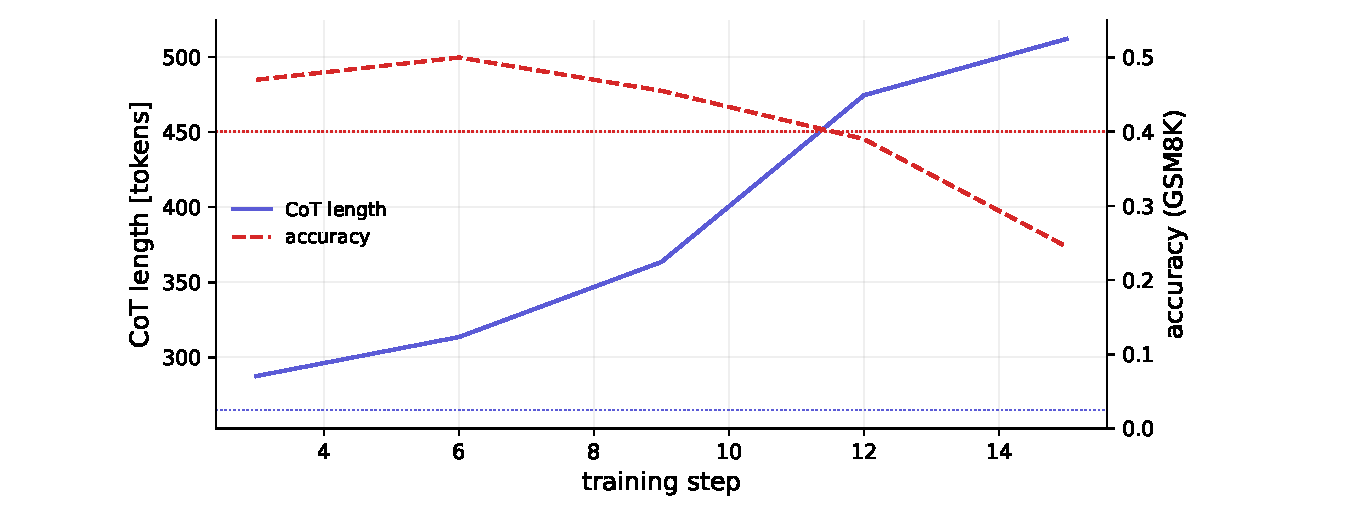
\includegraphics[width=\linewidth]{figures/fig_p2_neglambda.pdf}
  \caption{$\lambda = -0.05$. More doesn't mean better.}
  \label{fig:p2_neg}
\end{figure}

\begin{thebibliography}{99}

\bibitem{wei2022chain}
Jason Wei, Xuezhi Wang, Dale Schuurmans, Maarten Bosma, brian ichter, Fei Xia, Ed Chi,
Quoc V Le, and Denny Zhou. \href{https://arxiv.org/pdf/2201.11903}{Chain-of-Thought Prompting Elicits Reasoning in Large Language Models, 2022}. \textit{arXiv:2201.11903}

\bibitem{zhou2022least}
 Denny Zhou, Nathanael Schärli, Le Hou, Jason Wei, Nathan Scales, Xuezhi Wang, Dale Schuurmans, Claire Cui, Olivier Bousquet, Quoc V Le, and Ed H. Chi. \href{https://arxiv.org/pdf/2205.10625}{Least-to-Most Prompting Enables Complex Reasoning in Large Language Models, 2022}, \textit{arXiv:2205.10625}

\bibitem{fu2023complexity}
Yao Fu, Hao Peng, Ashish Sabharwal, Peter Clark, and Tushar Khot. \href{https://arxiv.org/pdf/2210.00720}{Complexity-based prompting for multi-step reasoning, 2023}. \textit{arXiv:2210.00720}

\bibitem{jin2024impact}
Mingyu Jin, Qinkai Yu, Dong Shu, Haiyan Zhao, Wenyue Hua, Yanda Meng, Yongfeng Zhang, and Mengnan Du. \href{https://arxiv.org/pdf/2401.04925}{The Impact of Reasoning Step Length on Large Language Models, 2024}. \textit{arXiv:2401.04925}

\bibitem{wu2025when}
Yuyang Wu, Yifei Wang, Ziyu Ye, Tianqi Du, Stefanie Jegelka, Yisen Wang. \href{https://arxiv.org/pdf/2502.07266}{When More is Less: Understanding Chain-of-Thought Length in LLMs, 2025}. \textit{arXiv:2502.07266}

\bibitem{skalse2022defining}
Joar Skalse, Nikolaus H. R. Howe, Dmitrii Krasheninnikov, David Krueger. \href{https://arxiv.org/pdf/2209.13085}{Defining and Characterizing Reward Hacking, 2022}. \textit{arXiv:2209.13085}

\bibitem{shao2024deepseekmath}
Zhihong Shao, Peiyi Wang, Qihao Zhu, Runxin Xu, Junxiao Song, Xiao Bi, Haowei Zhang, Mingchuan Zhang, Y.K. Li, Y. Wu, Daya Guo. \href{https://arxiv.org/pdf/2402.03300}{DeepSeekMath: Pushing the Limits of Mathematical
Reasoning in Open Language Models, 2024}. \textit{arXiv:2402.03300}

\bibitem{qwen2.5_technical_report}
Qwen Team et al. \href{https://arxiv.org/pdf/2412.15115}{Qwen2.5 Technical Report, 2024}. \textit{arXiv:2412.15115}

\bibitem{cobbe2021}
Cobbe, K., Kosaraju, V., Bavarian, M., et al. (2021). \href{https://arxiv.org/abs/2110.14168}{Training Verifiers to Solve Math Word Problems}. \textit{arXiv:2110.14168}.

\bibitem{tinyzero}
Jiayi Pan. \href{https://github.com/jiayipan/TinyZero}{TinyZero: A clean, minimal, and accessible implementation of DeepSeek-R1-Zero, 2025}. \textit{GitHub repository}

\bibitem{k3}
John Schulman. \href{http://joschu.net/blog/kl-approx.html}{Approximating KL Divergence
}. \textit{Web article}
\end{thebibliography}

\section*{Coding assistent usage}
A coding assistant (Claude) was used to generate the figures and to help write the RunPod launch scripts.


\end{document}